\chapter{Project Description}
		
		\textbf{\textit{dio 1. revizije}}\\
		
		\textit{Na osnovi projektnog zadatka detaljno opisati korisničke zahtjeve. Što jasnije opisati cilj projektnog zadatka, razraditi problematiku zadatka, dodati nove aspekte problema i potencijalnih rješenja. Očekuje se minimalno 3, a poželjno 4-5 stranica opisa.	Teme koje treba dodatno razraditi u ovom poglavlju su:}
		\begin{packed_item}
			\item \textit{potencijalna korist ovog projekta}
			\item \textit{postojeća slična rješenja (istražiti i ukratko opisati razlike u odnosu na zadani zadatak). Dodajte slike koja predočavaju slična rješenja.}
			\item \textit{skup korisnika koji bi mogao biti zainteresiran za ostvareno rješenje.}
			\item \textit{mogućnost prilagodbe rješenja }
			\item \textit{opseg projektnog zadatka}
			\item \textit{moguće nadogradnje projektnog zadatka}
		\end{packed_item}
		
		\textit{Za pomoć pogledati reference navedene u poglavlju „Popis literature“, a po potrebi konzultirati sadržaj na internetu koji nudi dobre smjernice u tom pogledu.}
		\eject
		
		\section{General Idea}
		\textit{The idea of this app is to enable a low to mid size festival organisation in a relatively simple and straight-forward manner that would be easily accessible and understandable even to non-technically educated Users.
		
		The application would be open-source, and would run on the Android OS - a native mobile app.}
		
		\section{Position in the market - the competition}
		\textit{Mainly, the competition consists of either high-profile professional apps, or non-native(non-mobile) apps. Thus, the point of this app is to fill that gap - it's supposed to be a native app, that's relatively simple to use, and very portable and easily deployable.}\\
		
		\textit{This would also imply, and goes hand in hand, with the fact that the application would be easy to use and easily accessible to a wide range of people - from highly-trained professional IT Users all the way to non-IT savvy amateur/inexperienced Users.}\\
		
		\textit{Because of the low difficulty, and relatively ad rem deployability, this app would be more suitable to the lower skill level(entry to mid-level) Users, as it is likely that Pro Users would require a larger scale App for, probably, larger caliber Festivals that they deal with. With that in mind however, this app can be used as a mini, mobile device reminder version of whatever Pro tool is used for Festival organisation.}\\
		
		\section{Primjeri u LaTeXu}
		
		\textit{Ovo potpoglavlje izbrisati.}\\

		U nastavku se nalaze različiti primjeri kako koristiti osnovne funkcionalnosti LaTeXa koje su potrebne za izradu dokumentacije. Za dodatnu pomoć obratiti se asistentu na projektu ili potražiti upute na sljedećim web sjedištima:
		\begin{itemize}
			\item Upute za izradu diplomskog rada u LaTeXu - \url{https://www.fer.unizg.hr/_download/repository/LaTeX-upute.pdf}
			\item LaTeX projekt - \url{https://www.latex-project.org/help/}
			\item StackExchange za Tex - \url{https://tex.stackexchange.com/}\\
		
		\end{itemize} 	


		
		%Ovo poglavlje je potrebno prilikom predaje obrisati
		
		\underbar{podcrtani tekst}, 
		\textbf{podebljani tekst}, 
		\textit{nagnuti tekst}\\
		\normalsize primjer
		\large primjer
		\Large primjer
		\LARGE {primjer}
		\huge {primjer}
		\Huge primjer
		\normalsize
				
		\begin{packed_item}
			
			\item  primjer
			\item  primjer
			\item  primjer
			\item[] \begin{packed_enum}
				
				\item primjer
				\item primjer
			\end{packed_enum}
			
		\end{packed_item}
		
		\noindent primjer url-a: \url{https://www.fer.unizg.hr/predmet/opp/projekt}
		
		
		\begin{longtabu} to \textwidth {|X[8, l]|X[8, l]|X[16, l]|} %definicija sirine polja
			
			\hline \multicolumn{3}{|c|}{\textbf{naslov unutar tablice}}	 \\[3pt] \hline
			\endfirsthead
			
			\hline \multicolumn{3}{|c|}{\textbf{naslov unutar tablice}}	 \\[3pt] \hline
			\endhead
			
			\hline 
			\endlastfoot
			
			\rowcolor{LightGreen}IDKorisnik & INT	&  	Lorem ipsum dolor sit amet, consectetur adipiscing elit, sed do eiusmod  	\\ \hline
			korisnickoIme	& VARCHAR &   	\\ \hline 
			email & VARCHAR &   \\ \hline 
			ime & VARCHAR	&  		\\ \hline 
			\cellcolor{LightBlue} primjer	& VARCHAR &   	\\ \hline 
			
			
		\end{longtabu}
		

		\begin{table}[H]
			
			
			
			\begin{longtabu} to \textwidth {|X[8, l]|X[8, l]|X[16, l]|} %definicija sirine polja
				
				\hline 
				\endfirsthead
				
				\hline 
				\endhead
				
				\hline 
				\endlastfoot
				
				\rowcolor{LightGreen}IDKorisnik & INT	&  	Lorem ipsum dolor sit amet, consectetur adipiscing elit, sed do eiusmod  	\\ \hline
				korisnickoIme	& VARCHAR &   	\\ \hline 
				email & VARCHAR &   \\ \hline 
				ime & VARCHAR	&  		\\ \hline 
				\cellcolor{LightBlue} primjer	& VARCHAR &   	\\ \hline 
				
				
			\end{longtabu}
	
			\caption{\label{tab:referencatablica} Naslov ispod tablice.}
		\end{table}
		
		\begin{figure}[H]
			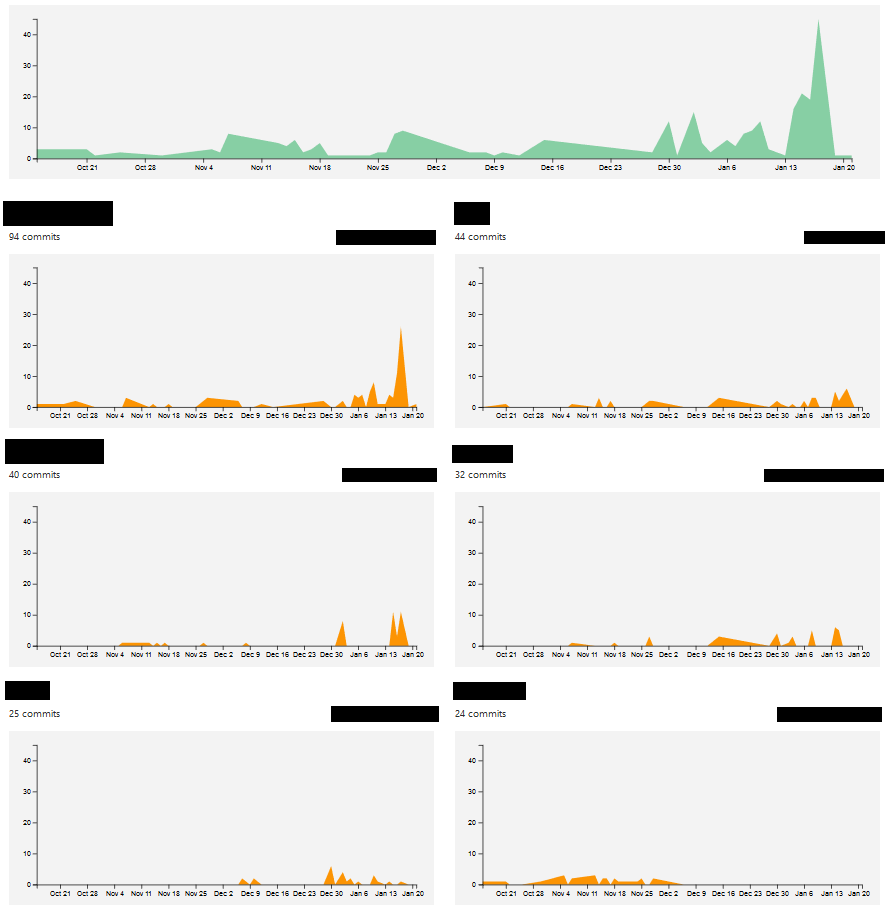
\includegraphics[scale=0.4]{slike/aktivnost.PNG}
			\centering
			\caption{Primjer slike s potpisom}
			\label{fig:promjene}
		\end{figure}
		
		\begin{figure}[H]
			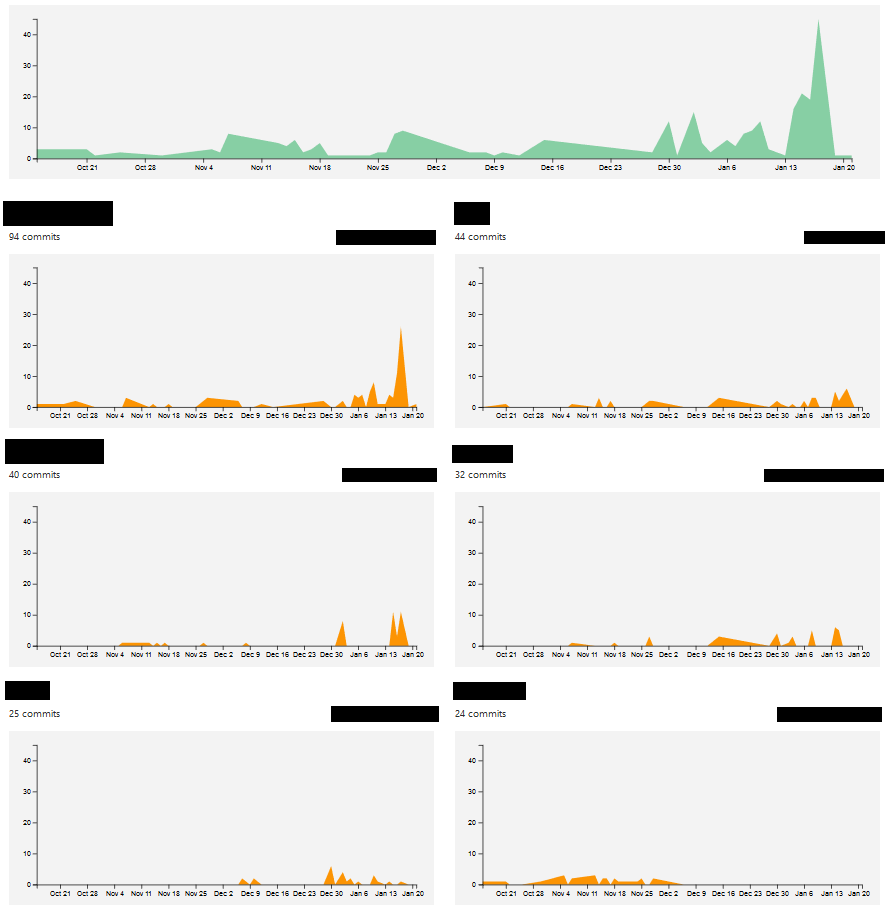
\includegraphics[width=\linewidth]{slike/aktivnost.PNG}
			\caption{Primjer slike s potpisom 2}
			\label{fig:promjene2}
		\end{figure}
		
		
		
		\eject
		
	